


\tikzset{every picture/.style={line width=0.75pt}} %set default line width to 0.75pt        

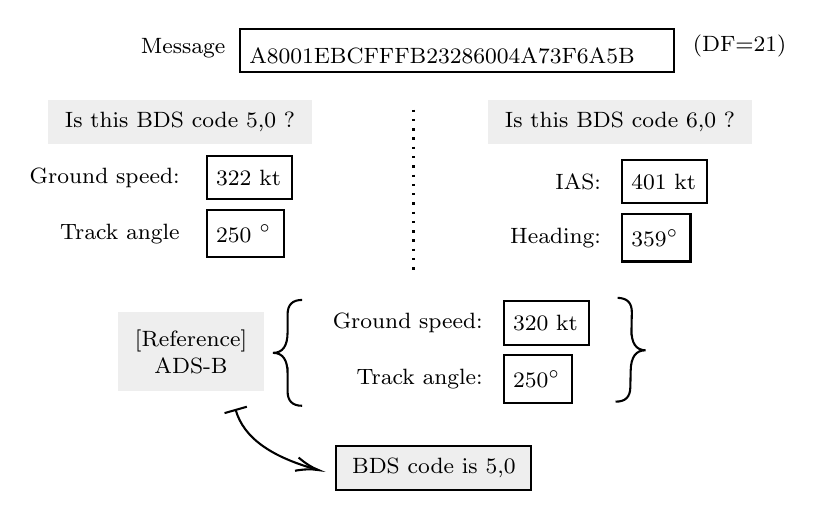
\begin{tikzpicture}[x=0.75pt,y=0.75pt,yscale=-1,xscale=1]
%uncomment if require: \path (0,348); %set diagram left start at 0, and has height of 348

%Straight Lines [id:da35241177696500303] 
\draw  [dash pattern={on 0.84pt off 2.51pt}]  (222.67,55.33) -- (222.67,133) ;
%Shape: Brace [id:dp1530573936144315] 
\draw   (169,147) .. controls (164.33,147) and (162,149.33) .. (162,154) -- (162,162.5) .. controls (162,169.17) and (159.67,172.5) .. (155,172.5) .. controls (159.67,172.5) and (162,175.83) .. (162,182.5)(162,179.5) -- (162,191) .. controls (162,195.67) and (164.33,198) .. (169,198) ;
%Shape: Brace [id:dp6255606362271318] 
\draw   (320,196) .. controls (324.67,196.09) and (327.05,193.81) .. (327.14,189.14) -- (327.3,181.14) .. controls (327.43,174.47) and (329.83,171.19) .. (334.5,171.28) .. controls (329.83,171.19) and (327.57,167.81) .. (327.7,161.14)(327.64,164.14) -- (327.86,153.14) .. controls (327.95,148.47) and (325.67,146.09) .. (321,146) ;
%Curve Lines [id:da4952815160936861] 
\draw    (137,200) .. controls (140.9,213.65) and (154.31,222.55) .. (175.37,228.54) ;
\draw [shift={(177,229)}, rotate = 195.26] [color={rgb, 255:red, 0; green, 0; blue, 0 }  ][line width=0.75]    (10.93,-3.29) .. controls (6.95,-1.4) and (3.31,-0.3) .. (0,0) .. controls (3.31,0.3) and (6.95,1.4) .. (10.93,3.29)   ;
\draw [shift={(137,200)}, rotate = 254.05] [color={rgb, 255:red, 0; green, 0; blue, 0 }  ][line width=0.75]    (0,5.59) -- (0,-5.59)   ;

% Text Node
\draw    (139.07,16.33) -- (348.07,16.33) -- (348.07,37.33) -- (139.07,37.33) -- cycle  ;
\draw (142.07,26.83) node [anchor=west] [inner sep=0.75pt]  [font=\footnotesize] [align=left] {\begin{minipage}[lt]{139.17356pt}\setlength\topsep{0pt}
\begin{center}
A8001EBCFFFB23286004A73F6A5B
\end{center}

\end{minipage}};
% Text Node
\draw (133.51,25.83) node [anchor=east] [inner sep=0.75pt]  [font=\footnotesize] [align=left] {Message};
% Text Node
\draw    (123.12,77.5) -- (164.12,77.5) -- (164.12,98.5) -- (123.12,98.5) -- cycle  ;
\draw (126.12,88) node [anchor=west] [inner sep=0.75pt]  [font=\footnotesize] [align=left] {322 kt};
% Text Node
\draw (111.52,88) node [anchor=east] [inner sep=0.75pt]  [font=\footnotesize] [align=left] {Ground speed:};
% Text Node
\draw    (123.12,103.5) -- (160.12,103.5) -- (160.12,126.5) -- (123.12,126.5) -- cycle  ;
\draw (126.12,115) node [anchor=west] [inner sep=0.75pt]  [font=\footnotesize] [align=left] {250 $\displaystyle ^{\circ }$};
% Text Node
\draw (111.52,115) node [anchor=east] [inner sep=0.75pt]  [font=\footnotesize] [align=left] {Track angle};
% Text Node
\draw    (323.12,79.5) -- (364.12,79.5) -- (364.12,100.5) -- (323.12,100.5) -- cycle  ;
\draw (326.12,90) node [anchor=west] [inner sep=0.75pt]  [font=\footnotesize] [align=left] {401 kt};
% Text Node
\draw (314.52,90) node [anchor=east] [inner sep=0.75pt]  [font=\footnotesize] [align=left] {IAS:};
% Text Node
\draw    (323.12,105.5) -- (356.12,105.5) -- (356.12,128.5) -- (323.12,128.5) -- cycle  ;
\draw (326.12,117) node [anchor=west] [inner sep=0.75pt]  [font=\footnotesize] [align=left] {359$\displaystyle ^{\circ }$};
% Text Node
\draw (314.52,117) node [anchor=east] [inner sep=0.75pt]  [font=\footnotesize] [align=left] {Heading:};
% Text Node
\draw  [draw opacity=0][fill={rgb, 255:red, 238; green, 238; blue, 238 }  ,fill opacity=1 ]  (46.65,50.83) -- (173.65,50.83) -- (173.65,71.83) -- (46.65,71.83) -- cycle  ;
\draw (110.15,61.33) node  [font=\footnotesize] [align=left] {Is this BDS code 5,0 ?};
% Text Node
\draw  [draw opacity=0][fill={rgb, 255:red, 238; green, 238; blue, 238 }  ,fill opacity=1 ]  (258.65,50.83) -- (385.65,50.83) -- (385.65,71.83) -- (258.65,71.83) -- cycle  ;
\draw (322.15,61.33) node  [font=\footnotesize] [align=left] {Is this BDS code 6,0 ?};
% Text Node
\draw  [color={rgb, 255:red, 0; green, 0; blue, 0 }  ,draw opacity=1 ][fill={rgb, 255:red, 238; green, 238; blue, 238 }  ,fill opacity=1 ]  (185.48,217.5) -- (279.48,217.5) -- (279.48,238.5) -- (185.48,238.5) -- cycle  ;
\draw (232.48,228) node  [font=\footnotesize] [align=left] {BDS code is 5,0};
% Text Node
\draw (355.8,24.83) node [anchor=west] [inner sep=0.75pt]  [font=\footnotesize] [align=left] {(DF=21)};
% Text Node
\draw    (266.12,147.5) -- (307.12,147.5) -- (307.12,168.5) -- (266.12,168.5) -- cycle  ;
\draw (269.12,158) node [anchor=west] [inner sep=0.75pt]  [font=\footnotesize] [align=left] {320 kt};
% Text Node
\draw (257.52,158) node [anchor=east] [inner sep=0.75pt]  [font=\footnotesize] [align=left] {Ground speed:};
% Text Node
\draw    (266.12,173.5) -- (299.12,173.5) -- (299.12,196.5) -- (266.12,196.5) -- cycle  ;
\draw (269.12,185) node [anchor=west] [inner sep=0.75pt]  [font=\footnotesize] [align=left] {250$\displaystyle ^{\circ }$};
% Text Node
\draw (257.52,185) node [anchor=east] [inner sep=0.75pt]  [font=\footnotesize] [align=left] {Track angle:};
% Text Node
\draw  [draw opacity=0][fill={rgb, 255:red, 238; green, 238; blue, 238 }  ,fill opacity=1 ]  (80.48,153) -- (150.48,153) -- (150.48,191) -- (80.48,191) -- cycle  ;
\draw (115.48,172) node  [font=\footnotesize] [align=left] {\begin{minipage}[lt]{44.88pt}\setlength\topsep{0pt}
\begin{center}
[Reference]\\ADS-B
\end{center}

\end{minipage}};


\end{tikzpicture}
